% SPIGM @ ICML 2026 workshop camera-ready.
% Same body text as main.tex (NeurIPS submission); only the formatting differs:
% ICML 2026 two-column style, non-anonymous authors, workshop notice.
\documentclass{article}

\newif\ifarxiv
\arxivtrue   % camera-ready: non-anonymous, show code link and acknowledgements

% Recommended packages for figures and typesetting.
\usepackage{microtype}
\usepackage{graphicx}
\usepackage{subcaption}
\usepackage{booktabs}
\usepackage{hyperref}
\usepackage{url}

% Make hyperref and algorithmic work together better.
\providecommand{\theHalgorithm}{\arabic{algorithm}}

% Ensure LaTeX finds the ICML-provided style dependencies in ./icml2026/.
\makeatletter
\def\input@path{{icml2026/}}
\makeatother

% ICML 2026 style, camera-ready (accepted) mode: shows author names.
\usepackage[accepted]{icml2026}

\usepackage[utf8]{inputenc}
\usepackage[T1]{fontenc}
\usepackage{amsmath}
\usepackage{amsfonts}
\usepackage{amssymb}
\usepackage{nicefrac}
\usepackage{comment}

% Paper macros and shared commands.
% Keep newcommand/DeclareMathOperator definitions here.

\usepackage{xcolor}
\newcommand{\TODO}[1]{\textcolor{red}{\textbf{[TODO:} #1\textbf{]}}}


% Replace the ICML proceedings notice with the SPIGM workshop notice.
\makeatletter
\renewcommand{\ICML@appearing}{\textit{Structured Probabilistic Inference
\& Generative Modeling workshop at the $\mathit{43}^{rd}$ International
Conference on Machine Learning}, Seoul, South Korea, 2026.
Copyright 2026 by the author(s).}
\makeatother

% Workshop build flag: routes the two 1D Laplace figures to the appendix, as in
% the NeurIPS submission.  All figures span both columns.
\def\spigmversion{}

\icmltitlerunning{Flash-SD-KDE: Accelerating SD-KDE with Tensor Cores}

\begin{document}

\twocolumn[
\icmltitle{Flash-SD-KDE: Accelerating SD-KDE with Tensor Cores}

\begin{icmlauthorlist}
\icmlauthor{Elliot L. Epstein}{icme}
\icmlauthor{Rajat Vadiraj Dwaraknath}{icme}
\icmlauthor{John Winnicki}{icme}
\end{icmlauthorlist}

\icmlaffiliation{icme}{Institute for Computational and Mathematical
Engineering (ICME), Stanford University, Stanford, CA, USA}

\icmlcorrespondingauthor{Elliot L. Epstein}{epsteine@stanford.edu}

\icmlkeywords{Kernel Density Estimation, Score Debiasing, Tensor Cores,
SD-KDE, GPU Acceleration, Triton}

\vskip 0.3in
]

\printAffiliationsAndNotice{}

\begin{abstract}
Score-debiased kernel density estimation (SD-KDE) achieves improved asymptotic convergence rates over classical KDE, but its use of an empirical score has made it significantly slower in practice. 
We show that by re-ordering the SD-KDE computation to expose matrix-multiplication structure, Tensor Cores can be used to accelerate the GPU implementation. 
On a 32k-sample 16-dimensional problem, our approach runs up to $47\times$ faster than a strong SD-KDE GPU baseline and $3{,}300\times$ faster than scikit-learn's KDE. 
On a larger 1m-sample 16-dimensional task evaluated on 131k queries, Flash-SD-KDE completes in $2.3$ s on a single GPU, making score-debiased density estimation practical at previously infeasible scales.
\ifarxiv Code available at \url{https://github.com/Elliotepsteino/Flash-SD-KDE}.\else Code available in supplementary material.\fi

\end{abstract}

\section{Introduction}

Score-debiased kernel density estimation (SD-KDE)~\cite{epstein2025sdkde}
improves the statistical efficiency of standard kernel density estimators:
for sufficiently smooth densities, SD-KDE attains better bias and mean-squared
error rates than vanilla KDE while retaining a simple, nonparametric form.
In particular, SD-KDE achieves an asymptotic mean integrated squared error
(AMISE) of order $O(n^{-8/(d+8)})$, improving the convergence exponent
relative to the $O(n^{-4/(d+4)})$ rate of classical KDE tuned with
Silverman's rule of thumb.
These accuracy gains come with a significant computational drawback: the
empirical score used for debiasing introduces an additional $O(n^2)$ pass
over the data, so a naive implementation has roughly the same quadratic cost
as KDE itself but with a larger constant factor.

Given samples $x_i$ and a bandwidth $h$, a Gaussian KDE is
\[
  \hat p(x)
  =
  \frac{1}{n h}
  \sum_{i=1}^n
  \varphi\!\left(\frac{x - x_i}{h}\right),
\]
and SD-KDE forms debiased samples
$x_i^{\mathrm{SD}} = x_i + \tfrac{h^2}{2}\,\hat s(x_i)$ where
$\hat s$ is an estimate of the score.  In this work we always use an
empirical score computed from the KDE itself, i.e.\ no parametric model
for the underlying density is assumed.  Writing the KDE explicitly in terms
of the samples,
\[
  \hat p(x)
  =
  \frac{1}{n h}
  \sum_{i=1}^n
  \varphi\!\left(\frac{x - x_i}{h}\right),
\]
we estimate the score as
\[
  \hat s(x)
  =
  \frac{\partial_x \hat p(x)}{\hat p(x)}
  =
  \frac{\sum_{i=1}^n \bigl[-\tfrac{x - x_i}{h}\,\varphi\!\left(\tfrac{x - x_i}{h}\right)\bigr]}
       {h^2 \sum_{i=1}^n \varphi\!\left(\tfrac{x - x_i}{h}\right)}.
\]

\section{Related Work}
\label{sec:related}

\paragraph{Kernel density estimation.}
Kernel density estimation (KDE) is a classical nonparametric approach to density estimation that dates back to the foundational work of \citet{rosenblatt1956remarks} and \citet{parzen1962estimation}; modern treatments appear in standard references such as \citet{silverman1986density} and \citet{wand1995kernel}.
For smooth densities, KDE attains optimal nonparametric rates under appropriate bandwidth scaling, but in practice performance is highly sensitive to bandwidth selection.
Rules-of-thumb and plug-in procedures are widely used for their simplicity, but they are typically tuned to unimodal, near-Gaussian targets and can misbehave for multimodal or heavy-tailed distributions \citep{silverman1986density, botev2010diffusion}.
This sensitivity is particularly pronounced in moderate and high dimensions, where the bandwidth controls both statistical bias and the computational cost of evaluating kernels at scale.

\paragraph{Bias reduction and adaptive smoothing.}
A large body of work improves KDE accuracy by reducing leading-order bias or adapting the effective smoothing scale across the sample space.
One line of work constructs higher-order bias corrections by modifying kernels or combining estimators so that the dominant $O(h^2)$ bias term cancels, yielding $O(h^4)$ bias under additional smoothness assumptions \citep{fan1992bias, jones1997comparison}.
Another class of methods uses variable bandwidths that shrink in regions of high density and expand in the tails, improving adaptivity without committing to a parametric form \citep{abramson1982bandwidth, silverman1986density}.
Complementary to these ideas, diffusion-based estimators view density estimation through the lens of smoothing by a linear diffusion process, providing both adaptivity and a data-driven bandwidth selection mechanism \citep{botev2010diffusion}.
Score-debiased KDE (SD-KDE) \citep{epstein2025sdkde} fits into this landscape by using score information to correct the leading bias term while retaining a simple kernel estimator structure.
Our Laplace-corrected formulation can be seen as an explicit higher-order correction that removes the need to form an empirical score at evaluation time, trading additional kernel evaluations for improved numerical and computational behavior.

\paragraph{Score estimation and score-based modeling.}
The score function $\nabla_x \log p(x)$ is a central object in statistics and machine learning.
Score matching \citep{hyvarinen2005score} provides a way to fit unnormalized models by matching scores rather than likelihoods, and denoising score matching connects score estimation to learning denoisers \citep{vincent2011connection}.
More recently, score-based generative models learn scores of noise-perturbed data distributions with neural networks and sample via Langevin or SDE-based dynamics \citep{song2019generative, song2021sde, ho2020ddpm}.
These works typically target high-dimensional perceptual data and emphasize sampling or likelihood computation, whereas SD-KDE uses an explicit nonparametric density estimator and an analytically-defined score to improve pointwise density estimation.
Related to our setting, Stein-based score estimators recover score information from samples via identities that avoid explicit density evaluation \citep{li2017gradient}.
Our focus is complementary: we keep the statistical estimator fixed (SD-KDE and its Laplace variant) and address the practical bottleneck that arises when score-corrected estimators are deployed at large scale.

\paragraph{Fast evaluation of kernel sums and density models.}
The computational cost of KDE and related kernel methods is dominated by evaluating large Gaussian sums or kernel matrices.
Algorithmic accelerations include multipole and series-expansion methods such as the Fast Gauss Transform (FGT) \citep{greengard1991fast} and improved variants tailored to Gaussian kernels \citep{yang2003improved}.
%, as well as space-partitioning and dual-tree methods for generic ``$N$-body'' statistical computations \citep{gray2001nbody, gray2003nonparametric}.
A different set of approaches uses randomized low-rank approximations (e.g., random Fourier features) to trade bias for computational efficiency \citep{rahimi2007random}.
These methods reduce asymptotic complexity but can be sensitive to dimensionality, bandwidth, and target accuracy.
In contrast, our work targets the exact SD-KDE computation and focuses on constant-factor reductions that make the estimator practical on modern accelerators.

\paragraph{GPU acceleration and tensor-core programming.}
A growing ecosystem of libraries and DSLs targets large kernel computations on GPUs.
KeOps provides a memory-efficient reduction framework for kernel and distance matrices and is a strong baseline for Gaussian kernel reductions at scale \citep{charlier2021keops}.
General deep learning frameworks such as PyTorch \citep{paszke2019pytorch} make it easy to express quadratic kernel computations, but their performance depends critically on whether the computation can be lowered to high-throughput primitives.
Domain-specific languages such as Triton \citep{tillet2019triton} enable writing custom GPU kernels while still benefiting from compiler support for tiling and scheduling.
At the hardware level, modern GPUs provide specialized matrix-multiply units (Tensor Cores) and mixed-precision execution paths that can offer large throughput improvements when computations are expressed in GEMM-like form \citep{micikevicius2017mixed, williams2009roofline}.
Recent ``flash''-style algorithms demonstrate that reordering computations to avoid materializing large intermediate matrices and to match the GPU memory hierarchy can yield substantial speedups for quadratic primitives \citep{dao2022flashattention}.
Our contribution follows this direction for score-corrected density estimation: we reorder SD-KDE to expose matrix-multiplication structure and implement a streaming accumulation strategy so that Tensor Cores can be used effectively without incurring prohibitive memory traffic.

\section{Hardware}
\label{sec:hardware}
\begin{figure*}[t]
  \centering
  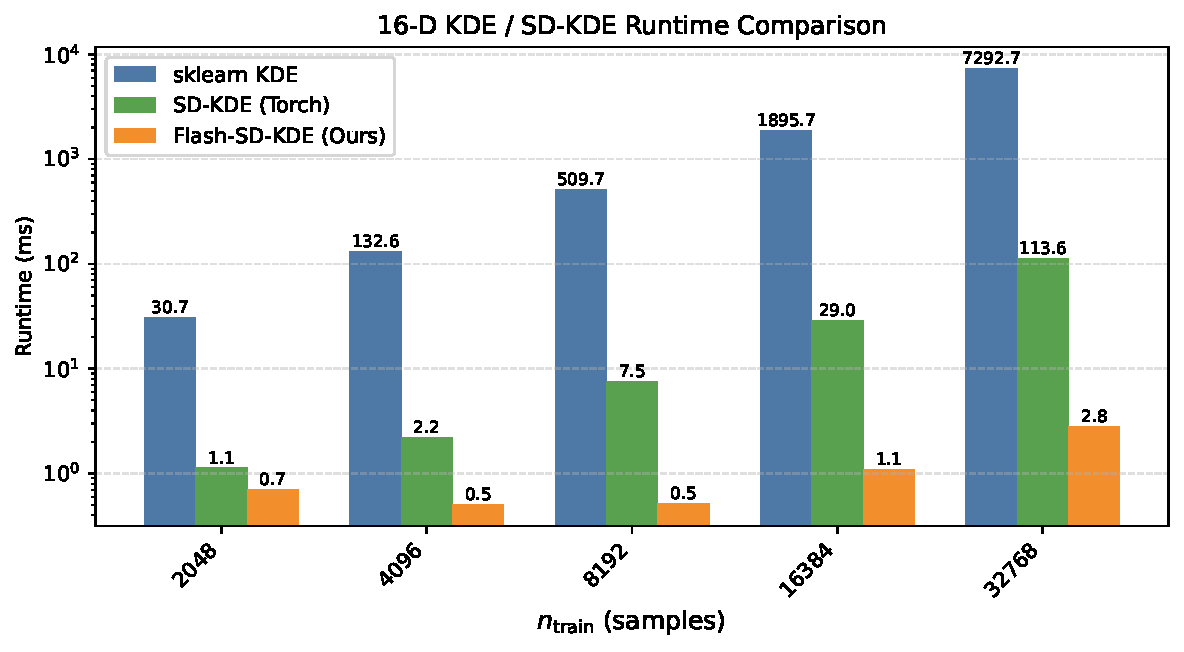
\includegraphics[width=\textwidth]{figures/runtime_16d_kde_sdkde.pdf}
  \caption{Runtime comparison for 16-D KDE/SD-KDE across $n_{\text{train}}$
           up to $32{,}768$ ($n_{\text{test}} = n_{\text{train}}/8$).}
  \label{fig:nd_runtime}
\end{figure*}
All experiments run on a workstation equipped with an NVIDIA RTX~A6000
(GA102).  This GPU exposes 84 streaming multiprocessors (SMs); each SM
contains 128 FP32 ALUs and 16 special function units (SFUs).  Because the
ratio of FP32 ALUs to SFUs is $128{:}16$, we treat one $\exp$ (issued on an
SFU) as costing the equivalent of $128/16 = 8$ FP32 flops in our models.
The card delivers roughly $40$~TFLOP/s of peak FP32 throughput and
approximately $770$~GB/s of GDDR6 bandwidth.

The host CPU is a dual-socket AMD EPYC~7763 system (``Milan'') configured
with $2 \times 64$ cores and two hardware threads per core (256 logical
CPUs reported by \texttt{lscpu}).  The processors boost up to
3.53~GHz, expose 512~MiB of shared L3 cache across the sockets, and provide
modern ISA extensions (AVX/AVX2, FMA, BMI1/2, SHA, VAES, etc.).

\section{Method}
\label{sec:method}

Our goal is to take $n_{\text{train}}$ samples in $d$ dimensions, form the
empirical SD-KDE (score + shift), and evaluate the resulting density on
$n_{\text{test}}$ queries.  Writing the computation in matrix form highlights
the parallel structure.  Let $x_i, y_j \in \mathbb{R}^d$ denote training and
query points, with bandwidth $h$ and squared Euclidean distance
\[
  \lVert x_i - y_j \rVert^2
  =
  \lVert x_i \rVert^2
  +
  \lVert y_j \rVert^2
  - 2\,x_i^\top y_j.
\]
Stacking training samples into $X \in \mathbb{R}^{n_{\text{train}}\times d}$
and queries into $Y \in \mathbb{R}^{n_{\text{test}}\times d}$, the
pairwise dot-product matrix
\[
  G
  =
  X Y^\top
  \in
  \mathbb{R}^{n_{\text{train}}\times n_{\text{test}}}
\]
dominates the arithmetic once $d$ is moderately large ($d\gtrsim 16$).  On
modern NVIDIA GPUs this GEMM can be mapped to Tensor Cores and evaluated at
5--10$\times$ the throughput of standard FP32 SIMT arithmetic, particularly
when we restrict to $d$ that are multiples of 16 and use Triton's
\texttt{tl.dot} interface.  The remaining operations---vector norms,
broadcasted additions, and exponentials---are all $O(n_{\text{train}}
 n_{\text{test}})$ but quickly become a small fraction of the total FLOPs as
$d$ grows.

The empirical SD-KDE score inherits the same GEMM structure.  Its numerator
involves terms of the form
\[
  \sum_j -(x_i - y_j)\,\varphi_{ij},
  \qquad
  \varphi_{ij}
  = \exp\!\left(-\frac{\lVert x_i - y_j\rVert^2}{2h^2}\right),
\]
which naively suggests $O(n_{\text{train}} n_{\text{test}} d)$ additional
elementwise arithmetic.  Using the identity
\[
  \sum_j (x_i - y_j)\,\varphi_{ij}
  =
  x_i \sum_j \varphi_{ij}
  -
  \sum_j \varphi_{ij}\,y_j,
\]
we can decompose the numerator into a second GEMM:
\[
  T
  =
  \Phi Y.
\]
Thus both the KDE evaluation and the SD-KDE score numerator reduce to
Tensor-Core-accelerable matrix multiplies, plus $O(n^2)$ scalar work for the
norms and exponentials.  In this note we focus on the $d=16$ case, which
aligns naturally with the Tensor Core tile sizes on the RTX~A6000.

\subsection{Arithmetic intensity in $d$ dimensions}

To understand when the high-dimensional SD-KDE becomes compute-bound, we
estimate FLOPs, bytes moved, and arithmetic intensity for the $d$-dimensional
case.  Let $n_{\text{train}} = k$ and set $n_{\text{test}} = k/8$ as in the
experiments.

\paragraph{Total FLOPs.}
The 16-D implementation consists of three main matrix-multiply stages:
\begin{enumerate}
  \item Score Gram matrix $G = X X^\top$:
        $2 d k^2$ FLOPs.
  \item Score numerator $T = \Phi X$:
        $2 d k^2$ FLOPs, plus $4 k^2$ scalar FLOPs for norms and distance
        terms and $8 k^2$ FLOPs for exponentials (counting each $\exp$ as
        $8$ FLOPs due to the SFU/FP32 ratio).
  \item Final KDE Gram matrix on debiased data:
        $2 d k (k/8)$ FLOPs, plus $4 k (k/8)$ scalar FLOPs and
        $8 k (k/8)$ FLOPs for exponentials.
\end{enumerate}
Aggregating these terms yields
\[
  \begin{aligned}
    \text{FLOPs}_d(k)
    &\approx
    4 d k^2 + 12 k^2 + 2 d \frac{k^2}{8} + 12 \frac{k^2}{8} \\
    &=
    \Bigl(4 d + 12 + \tfrac{d}{4} + \tfrac{3}{2}\Bigr) k^2.
  \end{aligned}
\]
Substituting $d=16$ gives
\[
  \text{FLOPs}_{16}(k)
  \approx
  81.5\,k^2,
\]
which is on the order of $10^{11}$ FLOPs for $k=32\text{k}$.

\paragraph{Bytes moved.}
To better capture implementation details, we count bytes per tile using the
launch parameters that delivered the best runtime ($BLOCK\_M = 64$,
$BLOCK\_N = 1024$).  Each tile loads $64\times d$ query values once
($4\,BLOCK\_M d$ bytes), streams $1024\times d$ training values
($4\,BLOCK\_N d$ bytes), and writes the partial PDF and weighted sums
($4\,BLOCK\_M$ and $4\,BLOCK\_M d$ bytes).  All of this traffic goes to and from
GDDR6, so for $d=16$ a tile moves roughly
\[
  \begin{aligned}
    \text{Bytes}_{\text{tile}}
    &\approx
    4\bigl(BLOCK\_M d + BLOCK\_N d \\
    &\qquad + BLOCK\_M + BLOCK\_M d\bigr) \\
    &= 4\bigl(2\,BLOCK\_M d + BLOCK\_N d \\
    &\qquad + BLOCK\_M\bigr) \\
    &\approx 7.4\times 10^4\ \text{bytes}.
  \end{aligned}
\]
The full problem processes $(k / BLOCK\_M)\times(k / BLOCK\_N)$ such tiles,
so the total GDDR6 traffic is
\[
  \begin{aligned}
    \text{Bytes}_{16}(k)
    &\approx
    \text{Bytes}_{\text{tile}}
    \times
    \frac{k}{BLOCK\_M}
    \times
    \frac{k}{BLOCK\_N} \\
    &\approx
    1.13\,k^2\ \text{bytes}.
  \end{aligned}
\]

\paragraph{Arithmetic intensity.}
Dividing FLOPs by bytes gives
\[
  \begin{aligned}
    I_d(k)
    &=
    \frac{\text{FLOPs}_d(k)}{\text{Bytes}_d(k)} \\
    &\approx
    \frac{\bigl(4 d + 12 + \tfrac{d}{4} + \tfrac{3}{2}\bigr) k^2}
         {4\bigl(\tfrac{9}{8} d k + \tfrac{k}{8}\bigr)} \\
    &\sim
    C(d)\,k
    \quad\text{for large }k,
  \end{aligned}
\]
with
\[
  C(d)
  \approx
  \frac{4 d + 12 + d/4 + 3/2}{4\cdot (9 d/8)}
  =
  \frac{(17/4)\,d + 27/2}{9 d/2}.
\]
For $d=16$ this simplifies to
\[
  I_{16}(k)
  \approx
  \frac{\text{FLOPs}_{16}(k)}{\text{Bytes}_{16}(k)}
  \approx
  \frac{81.5\,k^2}{1.13\,k^2}
  \approx 72\ \text{flops/byte}.
\]
This tile-aware estimate more closely reflects the measured arithmetic
intensity.  Comparing against the A6000 specs (Tensor Core peak of
$155\,\text{TFLOP/s}$ versus $\approx 770\,\text{GB/s}$ of memory bandwidth),
the machine balance is roughly $200$ flops/byte.  Since our kernel sustains
over $70$ flops/byte, it lies well into the compute-bound regime on the
RTX~A6000.  Nsight Compute reports an empirical arithmetic intensity of roughly
$95\,\text{FLOPs/byte}$ for the score kernel on the A6000, which is broadly in
line with the $72\,\text{FLOPs/byte}$ predicted by the tile-level model above.
Minor differences stem from additional bookkeeping work (atomics, reductions)
and from Nsight's finer-grained accounting of texture/cache traffic, but both
figures agree that the kernel operates far above the bandwidth roofline.
Because the kernel mixes Tensor-Core GEMMs with FP32 scalar work (norms,
exponentials, atomics), the effective machine balance sits between the
tensor-core roof ($\approx 200$ flops/byte) and the FP32 roof ($\approx 50$
flops/byte).  The observed $70$--$95$ flops/byte therefore straddle these two
limits: the GEMM portion is partially bandwidth-limited relative to Tensor
Cores, while the scalar portion is compute-limited relative to FP32 ALUs.

\section{Laplace-corrected KDE}
\label{sec:laplace_corrected}

Score-debiased KDE offers better asymptotic error rates, but its empirical score step adds a full quadratic pass over the data.
A natural approximation is to replace the explicit debiasing with a correction to the kernel itself.
This yields a Laplace-corrected KDE that captures the leading-order bias reduction of SD-KDE while avoiding the empirical score computation.

Let $K_h(x)$ denote the isotropic Gaussian kernel in $d$ dimensions.
\[
  K_h(x)
  =
  \frac{1}{(2\pi)^{d/2} h^d}
  \exp\!\left(-\frac{\lVert x \rVert^2}{2h^2}\right),
\]
Let $\hat p(x) = \tfrac{1}{n} \sum_i K_h(x - x_i)$ be the corresponding KDE.
The Laplace-corrected kernel is defined by
\[
  K_h^{\text{LC}}(x)
  =
  K_h(x) - \frac{h^2}{2} \Delta K_h(x).
\]
For the Gaussian kernel, the Laplacian has a closed form.
\[
  K_h^{\text{LC}}(x)
  =
  K_h(x)\left(1 + \frac{d}{2} - \frac{\lVert x \rVert^2}{2h^2}\right),
\]
The estimator becomes
\[
  \hat p_{\text{LC}}(x)
  =
  \frac{1}{n} \sum_{i=1}^n K_h^{\text{LC}}(x - x_i).
\]

\paragraph{Connection to SD-KDE.}
SD-KDE forms debiased samples $x_i^{\text{SD}} = x_i + \tfrac{h^2}{2}\,\hat s(x_i)$ using an empirical score $\hat s$.
Evaluating a KDE on the shifted samples and linearizing in $h^2$ yields a correction proportional to $\Delta K_h$.
When $\hat s$ is taken to be the KDE score, this linearized estimator coincides with the Laplace-corrected kernel above.
Thus $\hat p_{\text{LC}}$ can be viewed as a first-order approximation to SD-KDE that preserves its leading bias reduction while avoiding an explicit score pass.

\paragraph{Why we consider this correction.}
The Laplace-corrected estimator is appealing when the full SD-KDE score is too expensive or when a fast bias-reduction surrogate is sufficient.
It requires only the same pairwise distances and exponentials as standard KDE, plus a simple affine factor in the kernel value.
The correction can be negative for large $\lVert x - x_i \rVert$, so $\hat p_{\text{LC}}$ is not guaranteed to be nonnegative, which we account for in our experiments.

\paragraph{Kernel fusion opportunity.}
Computing $K_h^{\text{LC}}$ reuses the same scaled distances used to compute $K_h$.
A fused kernel can compute $\phi = \exp(-\tfrac{1}{2}\,\text{scaled})$ and apply the Laplace factor inside the same pass.
A non-fused implementation must either recompute distances or materialize intermediates in a second kernel.
This increases memory traffic and kernel launches.
We therefore treat the fused Laplace-corrected kernel as a distinct fast path and refer to it as \emph{Flash-SD-KDE}.

\section{Results}

We now summarize the empirical behavior of the 16-D implementation on the
RTX~A6000.  For each $n_{\text{train}}$ in $\{4\text{k}, 8\text{k}, 16\text{k},
32\text{k}\}$ we set $n_{\text{test}} = n_{\text{train}}/8$, draw data from a
simple 16-D Gaussian mixture, and run three baselines: scikit-learn KDE,
Torch SD-KDE (GEMM-based), and Triton SD-KDE (Tensor-Core GEMMs for both KDE
and score).  Figure~\ref{fig:nd_runtime} shows that the Triton SD-KDE rapidly
outpaces both baselines as $n$ grows, while remaining numerically close to the
Torch SD-KDE reference.

We also measure utilization by combining the flop model above with the
measured runtimes.  As shown in Figure~\ref{fig:triton_sd_kde_nd_util}, the
Torch SD-KDE baseline reaches only a few percent of the A6000 Tensor Core
peak, whereas the Triton implementation climbs into the multi-digit range once
$n_{\text{train}}$ exceeds $8\text{k}$.  This confirms that the 16-D
Tensor-Core formulation is firmly compute-bound and that additional tuning
effort should focus on kernel fusion and occupancy rather than memory traffic.

To compare against a specialized KDE implementation, we also benchmarked PyKeOps
LazyTensor operators at $n_{\text{train}}=32\text{k}$, $n_{\text{test}}=4\text{k}$.
PyKeOps currently represents the state of the art for large-scale kernel
reductions, so we report both its Gaussian KDE runtime and its SD-KDE runtime as
a reference point.  Table~\ref{tab:pykeops} shows that Triton SD-KDE runs
$1.4\times$ faster than the PyKeOps 16-D KDE baseline and $9.8\times$ faster
than the PyKeOps 16-D SD-KDE implementation.

\begin{table}[h]
  \centering
  \small
  \setlength{\tabcolsep}{4pt}
  \begin{tabular}{lcc}
    \toprule
    Method & Runtime (ms) & Rel to Triton \\
    \midrule
    Triton 16-D SD-KDE & $2.23$ & $1\times$ \\
    PyKeOps 16-D KDE   & $3.06$ & $1.4\times$ \\
    PyKeOps 16-D SD-KDE& $21.73$ & $9.77\times$ \\
    \bottomrule
  \end{tabular}
  \caption{Runtime comparison at $n_{\text{train}}=32\text{k}$,
           $n_{\text{test}}=4\text{k}$.  PyKeOps rows report Gaussian KDE and
           SD-KDE (LazyTensor) runtimes, while Triton executes the full SD-KDE
           pipeline.}
  \label{tab:pykeops}
\end{table}

\begin{figure*}[t]
  \centering
  
\includegraphics[width=\textwidth]{figures/nd-runtime.pdf}
  \caption{Runtime comparison for 16-D KDE/SD-KDE across $n_{\text{train}}$
           up to $32{,}768$ ($n_{\text{test}} = n_{\text{train}}/8$).}
  \label{fig:nd_runtime}
\end{figure*}

\subsection{Performance optimizations}
\begin{figure*}[t]
  \centering
  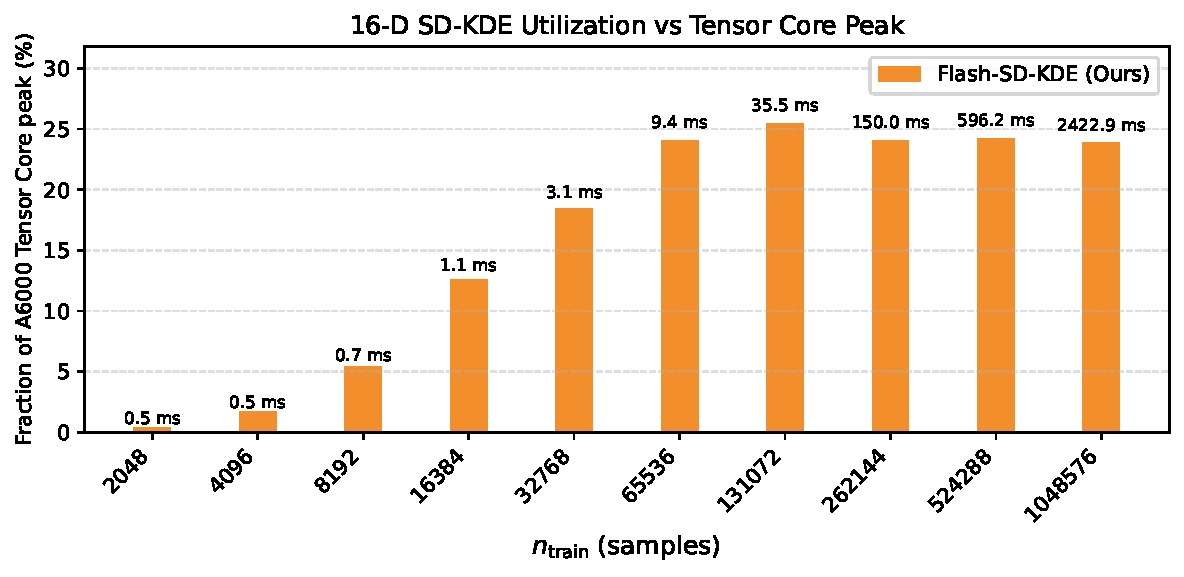
\includegraphics[width=0.9\textwidth]{figures/util_16d_sdkde_tensorcore.pdf}
  \caption{Utilization (percentage of RTX A6000 Tensor Core peak) for the 16-D
           SD-KDE pipeline, computed via the flop model from
           Section~\ref{sec:method}; bars are annotated with the observed
           runtimes (ms).}
  \label{fig:triton_sd_kde_nd_util}
\end{figure*}
% [MOVED TO Appendix~\ref{app:kernel_tuning}: The exact launch-parameter grid is reproducibility detail.  We keep the selected best configuration and effect size in the main text and move the full sweep description to Appendix~\ref{app:kernel_tuning}.]
\begin{comment}
Nsight Systems traces show that roughly $95\%$ of the SD-KDE runtime at
$n_{\text{train}}=32\text{k}$, $n_{\text{test}}=4\text{k}$ is spent computing
the empirical score.  We therefore concentrated optimization effort on the
score kernel, sweeping the launch parameters to raise utilization.  Specifically
we varied:
\begin{itemize}
  \item $BLOCK\_M \in \{32, 64, 128, 256\}$,
  \item $BLOCK\_N \in \{32, 64, 128, 256, 512, 1024\}$,
  \item $num\_warps \in \{1, 2, 4, 8\}$,
  \item $num\_stages \in \{1, 2, 4\}$,
\end{itemize}
and selected the combination that minimized runtime.  For this workload we
found that $BLOCK\_M=64$, $BLOCK\_N=1024$, $num\_warps=2$, and $num\_stages=2$
gave the best overall performance, increasing measured FLOP utilization by
more than $2\times$ relative to smaller-tile settings.
\end{comment}
% [END MOVED TO Appendix~\ref{app:kernel_tuning}]

% \begin{revadded}
Nsight Systems traces show that roughly $95\%$ of the SD-KDE runtime at $n_{\text{train}}=32\text{k}$, $n_{\text{test}}=4\text{k}$ is spent computing the empirical score.  We therefore tune the score-kernel launch configuration; the full grid is given in Appendix~\ref{app:kernel_tuning}.  The best setting uses $BLOCK\_M=64$, $BLOCK\_N=1024$, $num\_warps=2$, and $num\_stages=2$, increasing measured FLOP utilization by more than $2\times$ relative to smaller-tile settings.
% \end{revadded}

Beyond the launch-parameter sweep, two design choices account for most of the
speedup over a standard tiling implementation:
\begin{enumerate}
  \item \textbf{Tensor-Core tiling:} all high-dimensional dot products are
        processed as $16 \times 16$ tiles with Tensor Core
        acceleration, allowing the GEMM portion of the score and KDE kernels
        to run near the TF32 roofline.
  \item \textbf{Streaming accumulation:} we never materialize full
        $n_{\text{train}}\times n_{\text{train}}$ (or query) matrices; instead
        we stream tiles through registers and rely on atomic reductions to keep
        global-memory traffic linear in $n$.
\end{enumerate}

Appendices~\ref{app:streaming_ablation} and~\ref{app:tc_ablation} quantify the
factors.  At $n_{\text{train}}=65{,}536$ and
$n_{\text{test}}=8{,}192$, streaming reduces peak extra GPU allocation from
$\sim\!16$ GB to $\sim\!16$ MB and gives a $55.7\times$ speedup over
full materialization.  Holding the streamed implementation fixed, enabling
Tensor-Core tiling gives a $4.94\times$ speedup at
$n_{\text{train}}=32{,}768$ and remains near $5\times$ at the largest
sizes.  Thus streaming makes the exact quadratic computation fit in memory,
while Tensor Cores supply the large-$n$ throughput.

Together these optimizations push the kernels close to the hardware limit.
Nsight Compute's ``Speed of Light'' report shows $\sim 68\%$ SM throughput and
roughly $90\%$ L1 throughput for the score kernel at
$n_{\text{train}}=32\text{k}$ and $n_{\text{test}}=4\text{k}$, which is
consistent with the tensor-core utilization trends in
Figure~\ref{fig:triton_sd_kde_nd_util}: we cannot reach the nominal Tensor
Core peak because the kernel still executes substantial non-Tensor-Core work
(norms, exponentials, atomics).  At these utilization levels we stopped
further low-level tuning, since additional optimizations would likely yield
only modest incremental gains.












\section{Conclusion}
\label{sec:conclusion}
Score-debiased kernel density estimation (SD-KDE) offers improved asymptotic accuracy over classical KDE, but its reliance on an empirical score has historically made it substantially slower in practice. 
This paper shows that the dominant cost of empirical SD-KDE is not inherently prohibitive: by re-ordering the computation to expose matrix-multiplication structure, both KDE evaluation and the score numerator can be expressed as Tensor Core--accelerable GEMMs plus lightweight elementwise operations, while avoiding materializing full pairwise interaction matrices via streaming accumulation. 
In the 16-D setting, this hardware-aligned formulation yields large end-to-end gains---up to $47\times$ faster than a strong Torch SD-KDE baseline and $3{,}300\times$ faster than scikit-learn KDE---and scales to previously infeasible regimes, completing SD-KDE on $\sim$1M training points and $\sim$131k queries in 2.3\,s on a single GPU. 

 Overall, our results suggest that practical nonparametric estimators can often be unlocked by hardware-aware reformulations that maximize GPU utilization. 
 Future directions include extending the approach beyond $d$ multiples of 16, supporting richer bandwidth parameterizations and kernels, further reducing non-Tensor-Core overheads (e.g., exponentials and atomics), and developing nonnegativity-preserving approximations and multi-GPU variants.

\ifarxiv
\section*{Acknowledgements}

Large language models (LLMs) were used to assist both the implementation and
the preparation of this paper. LLMs helped with kernel prototyping,
refactoring, and drafting and editing text.

\fi
\input{sections/09_impact}

\bibliographystyle{icml2026}
\bibliography{references}


\section{Low-dimensional and Laplace-correction details}
\label{app:method_details}

\subsection{Flash-SD-KDE in low dimensions}

For completeness we briefly summarize the 1-D SD-KDE arithmetic intensity and
empirical behavior.  With $n_{\text{train}} = k$ and $n_{\text{test}} = k/8$,
there are two steps:
\begin{enumerate}
  \item \textbf{Score + shift:} For each training point we compute
        $\hat s(x_i)$ from all $k$ points and then form
        $x_i^{\mathrm{SD}} = x_i + \tfrac{h^2}{2}\hat s(x_i)$.  This uses
        $O(k^2)$ pairwise kernel interactions.  With the RTX~A6000 hardware
        ratio ($128$ FP32 ALUs, $16$ SFUs per SM) we budget an $\exp$ as
        $8$ flop-equivalents.  The score accumulation requires one $\exp$
        and roughly eight additional arithmetic ops (subtraction, scaling,
        accumulation), yielding $c_1 \approx 16$ flops per
        $(\text{train},\text{train})$ pair.
  \item \textbf{KDE on debiased samples:} We then evaluate a standard Gaussian
        KDE at $k/8$ query points using the $k$ debiased samples, which uses
        $O(k^2/8)$ interactions.  Each pair requires one $\exp$ (8 flops) plus
        about six other operations (difference, square, scaling, accumulation),
        so we take $c_2 \approx 14$ flops per $(\text{train},\text{test})$ pair.
\end{enumerate}
The total work is therefore approximated by
\[
  \text{FLOPs}(k)
  \;\approx\;
  c_1 k^2 + c_2\,k\,(k/8)
  \;\approx\;
  16 k^2 + 14\frac{k^2}{8}
  \;=\;
  17.75\,k^2.
\]
For $k = 32\text{k}$ this is on the order of $2\times 10^{10}$ flops.  When we
fix $n_{\text{test}} = k/8$ we move approximately $5k$ bytes (counting one
read of each train and test point and one write of each output), so the
arithmetic intensity scales as
\[
  I(k)
  =
  \frac{\text{FLOPs}(k)}{\text{Bytes}(k)}
  \;\approx\;
  \frac{17.75\,k^2}{5\,k}
  \approx
  3.55\,k
  \quad \text{flops/byte},
\]
placing realistic problem sizes firmly in the compute-bound regime.

Empirically we sweep $k$ over powers of two from $1024$ to $64\text{k}$, with
$n_{\text{test}} = k/8$, and average over three seeds.  For each
configuration we record scikit-learn Gaussian KDE
time, and SD-KDE Torch time, and Flash-SD-KDE time.  Across the entire range, the Flash-SD-KDE
implementation is consistently faster than scikit-learn, with speedups
growing with $k$; at the largest sizes, Flash-SD-KDE achieves around 2 orders-of-magnitude speedup relative to the sklearn baseline, as shown in Figure~\ref{fig:flash_sd_kde}.

\begin{figure*}[th]
  \centering
  
\includegraphics[width=0.8\linewidth]{figures/runtime_1d_kde_sdkde.pdf}
  \caption{Average runtime (log-scale $y$-axis) of scikit-learn KDE, SD-KDE (Torch), and Flash-SD-KDE across $n_{\text{train}}$ in 1-D; annotations show observed runtimes.}
  \label{fig:flash_sd_kde}
\end{figure*}

%\begin{figure}[th]
%  \centering
%  \includegraphics[width=0.8\linewidth]{figures/emp-sd-kde-%util.pdf}
%  \caption{Estimated GPU utilization (as a percentage of A6000 %FP32 peak)
%           for 1-D SD-KDE implemented in Triton and optimized %Torch,
%           computed from the 1-D flop model and the measured %runtimes.}
%  \label{fig:flash_sd_kde_util}
%\end{figure}

As shown in Figure~\ref{fig:triton_large_util}, we also compare the utilization of Flash-SD-KDE with SD-KDE (Torch) over a range of 1-D problem sizes, using powers of
two for $n_{\text{train}}$ up to $2^{16} \approx 64$ thousand (and
$n_{\text{test}} = n_{\text{train}}/8$).  

\begin{figure*}[th]
  \centering
  
\includegraphics[width=0.8\linewidth]{figures/util_1d_empirical_sdkde.pdf}
  \caption{Utilization of the 1-D Flash-SD-KDE kernel and SD-KDE (Torch) for large
           $n_{\text{train}}$ (powers of two up to $2^{16}$).  Labels show
           the observed runtime for each data size; error bars are omitted
           because a single seed is used per point.}
  \label{fig:triton_large_util}
\end{figure*}


\begin{comment}
\section{Oracle density benchmark for Laplace correction beyond $10^6$}
\label{sec:laplace_corrected}
The results are shown below.
\begin{figure*}[t]
  \centering
  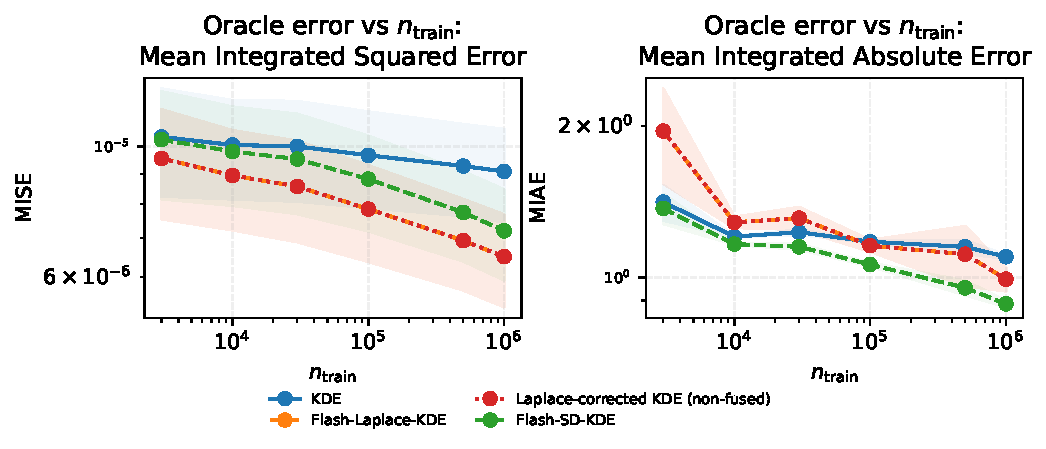
\includegraphics[width=\textwidth]{figures/fig_oracle_error_vs_n_16d.pdf}
  \caption{Oracle error on a 16D mixture-of-Gaussians benchmark.
           We report MISE and MIAE versus $n_{\text{train}}$ for KDE and Flash-Laplace-KDE (fused Laplace correction).}
  \label{fig:e6_fig_oracle_error_vs_n}
\end{figure*}
\end{comment}


% \begin{revadded}
\subsection{Laplace-corrected KDE derivation and 1D benchmarks}
\label{app:laplace_derivation}

% \end{revadded}

% [RED WRAP MOVED LAPLACE FIGURES]
\begin{revadded}
\begin{figure*}[t]
  \centering
  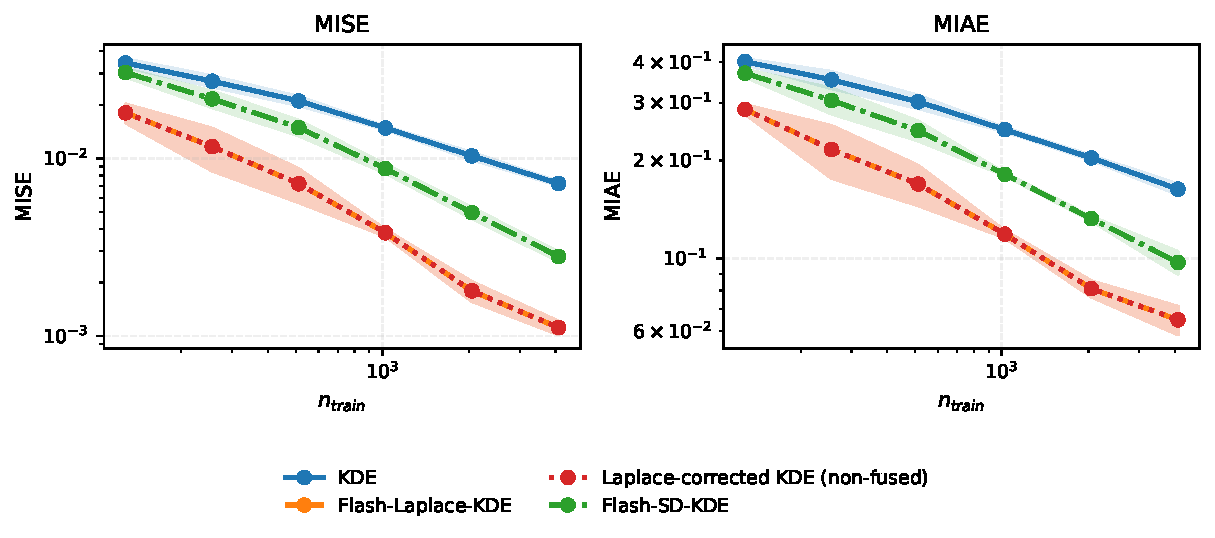
\includegraphics[width=\textwidth]{figures/fig_oracle_error_vs_n_1d.pdf}
  \caption{Oracle error on a 1D mixture-of-Gaussians benchmark.
           We report MISE and MIAE versus $n_{\text{train}}$ for KDE, Flash-Laplace-KDE (fused Laplace correction), non-fused Laplace correction, and Flash-SD-KDE.
           The Laplace-corrected estimators can be slightly negative, so error is computed on the signed density.}
  \label{fig:oracle_error_1d}
\end{figure*}

\begin{figure*}[t]
  \centering
  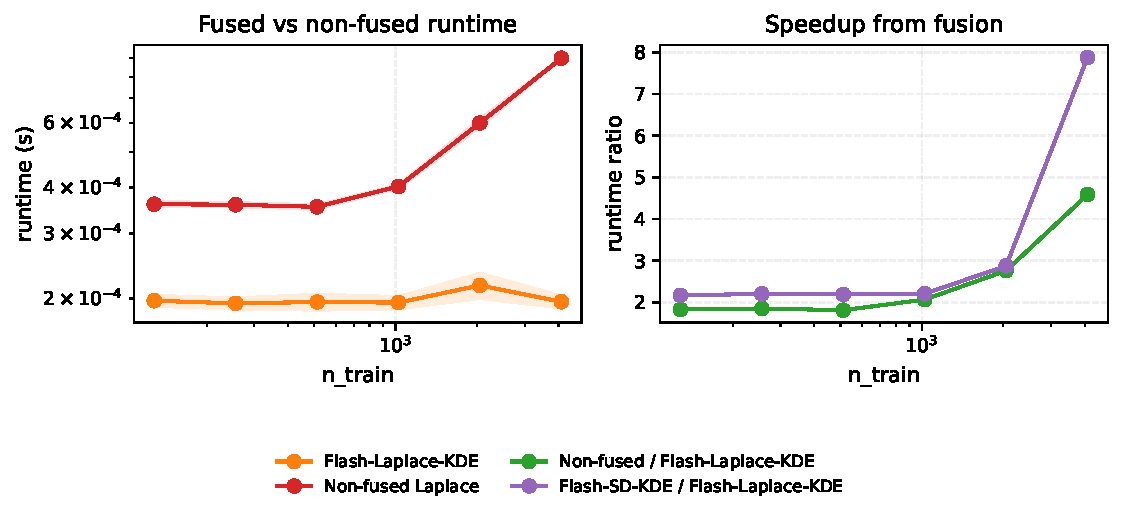
\includegraphics[width=\textwidth]{figures/fig_fused_vs_nonfused_runtime.pdf}
  \caption{Runtime and speedup for Laplace correction in 1D.
           The left panel shows total runtime for the fused Flash-Laplace-KDE kernel and a non-fused implementation.
           The right panel reports speedup ratios, including Flash-SD-KDE relative to Flash-Laplace-KDE for context.}
  \label{fig:laplace_speedup_1d}
\end{figure*}

\end{revadded}
% [END RED WRAP MOVED LAPLACE FIGURES]

% \begin{revadded}
We evaluate Laplace-corrected KDE on a 1D oracle density.
Figure~\ref{fig:oracle_error_1d} compares KDE, Flash-Laplace-KDE (fused Laplace correction), non-fused Laplace correction, and Flash-SD-KDE.
The Laplace-corrected estimators can take small negative values for large $\lVert x - x_i \rVert$.
We therefore compute errors on the signed density, and we report the negative-mass diagnostics separately in the benchmark logs.

Figure~\ref{fig:laplace_speedup_1d} shows the runtime advantage of fusion.
The fused Flash-Laplace-KDE kernel consistently outperforms the non-fused Laplace correction across $n_{\text{train}}$.
For context, the same plot also reports the Flash-SD-KDE to Flash-Laplace-KDE runtime ratio.

As an intuitive explanation of why both methods achieve the same leading bias reduction, we can first view vanilla KDE\footnote{Throughout, we assume that the kernel is Gaussian for simplicity.} as a heat semigroup (kernel) $P_{t} = e^{\frac{t}{2}\Delta}$ with $t = h^2$ applying to the empirical density  function $f_n$ (sampled with replacement) to be
\begin{align*}
    \hat{f} = P_t f_n.
\end{align*}
From the linearity of the heat semigroup, we then have that the expected estimate
\begin{align*}
    \mathbb{E}\left[\hat{f}\right]
    =\mathbb{E}\left[P_t f_n\right]
    =P_t\mathbb{E}\left[ f_n\right]
    =P_tf,
\end{align*}
where $f$ is the true probability density function.

The bias is then, under a smoothness assumption we assume throughout,
\begin{align*}
    \mathbb{E}\left[\hat{f}\right]-f = (P_t-I)f = \frac{t}{2} \Delta f + O(t^2).
\end{align*}

The Laplace kernel deals with this leading term by using an operator $\left(I-\frac{t}{2}\Delta\right)P_t$ instead, making its bias
\begin{align*}
    \mathbb{E}\left[\hat{f}^{\text{LC}}\right]-f = \left[\left(I-\frac{t}{2}\Delta\right)P_t-I\right]f = O(t^2).
\end{align*}

The SD-KDE algorithm approaches this debias task differently by applying a \textbf{non-linear}\footnote{Even when the transportation kernel has a non-linear transportation. The kernel itself is linear.} transportation kernel $T_{\frac{t}{2}\nabla \log f}$ before applying a standard heat kernel $P_t$, making its bias
\begin{align*}
    &\mathbb{E}\left[\hat{f}^{\text{SD-KDE}}\right]-f\\ &= \left[P_tT_{\frac{t}{2}\nabla f}-I\right]f\\
    &=
    \left[P_t\left(f - \frac{t}{2}\nabla \cdot \left(f\nabla \log f\right) + O(t^2)\right)-f\right]\\
    &=
    \left[P_t\left(f - \frac{t}{2}\Delta f + O(t^2)\right)-f\right]\\
    &=
    \left[P_t\left(I - \frac{t}{2}\Delta  \right)-I\right]f+ O(t^2)\\
    &= O(t^2).
\end{align*}
Recall that $t=h^2$, so we have that Laplace KDE and SD-KDE have an $O(h^4)$ bias, while vanilla KDE has an $O(h^2)$ bias.

Note that the analysis above assumes that the SD-KDE has access to the oracle, so the translation kernel is linear. In practice, the score is empirical, making the translation kernel
\begin{align*}
    T_{\frac{t}{2}\nabla \log \left(P_{t'} f_n\right)}
\end{align*}
where $t'=\frac{h^2}{2}$ is the bandwidth for the kernel used for score estimation. Thus, the empirical SD-KDE is
\begin{align*}
    \hat{f}^{\text{Emp SD-KDE}} = T_{\frac{t}{2}\nabla \log \left(P_{t'} f_n\right)} f_n,
\end{align*}
which is no longer linear in $f_n$.
% \end{revadded}

\section{Additional Experiments}
\label{app:additional}

This appendix reports additional measurements that complement the
benchmarks in Section~\ref{sec:results}.
We extend the runtime sweep to stronger exact baselines and to a second GPU,
isolate the contributions of streaming and Tensor-Core tiling through
controlled ablations, and evaluate Flash-SD-KDE on a real-data anomaly
detection benchmark.
All measurements use the 16-D pipeline.
Unless stated otherwise, runtimes are reported in milliseconds, exclude
one-time warmup and JIT compilation costs, and use the 16-D Gaussian-mixture
benchmark of Section~\ref{sec:results} with $n_{\text{test}} = n_{\text{train}}/8$.

\subsection{Extended baseline sweep on the RTX A6000}
\label{app:baseline_sweep}

To place Flash-SD-KDE against a fuller set of exact baselines, we extend the
PyKeOps comparison from a single point to the full $n_{\text{train}}$ sweep
and add a \texttt{torch.compile} variant of the GEMM-based PyTorch baseline.
Table~\ref{tab:rebuttal_baseline_sweep} reports runtimes on the RTX A6000.

\begin{table*}[t]
  \centering
  \small
  \setlength{\tabcolsep}{4pt}
  \begin{tabular}{rrrrrrr}
    \toprule
    $n_{\text{train}}$ & $n_{\text{test}}$ &
    sklearn & Torch & \texttt{torch.compile} & PyKeOps & Flash-SD-KDE \\
    \midrule
    $2{,}048$  & $256$  & $30.7$    & $1.1$   & $6.0$  & $1.9$  & $0.7$ \\
    $4{,}096$  & $512$  & $132.6$   & $2.2$   & $2.9$  & $2.5$  & $0.5$ \\
    $8{,}192$  & $1{,}024$ & $509.7$   & $7.5$   & $5.0$  & $3.6$  & $0.5$ \\
    $16{,}384$ & $2{,}048$ & $1{,}895.7$ & $29.0$  & $11.3$ & $6.7$  & $1.1$ \\
    $32{,}768$ & $4{,}096$ & $7{,}292.7$ & $113.6$ & $34.3$ & $21.7$ & $2.8$ \\
    \bottomrule
  \end{tabular}
  \caption{Average per-call runtime (ms) of exact 16-D SD-KDE implementations
           on the RTX~A6000, lower is better.
           Columns are scikit-learn Gaussian KDE, the GEMM-based PyTorch
           SD-KDE, the same PyTorch implementation under
           \texttt{torch.compile}, the PyKeOps LazyTensor SD-KDE, and our
           Flash-SD-KDE.
           Data are drawn from the 16-D Gaussian-mixture benchmark of
           Section~\ref{sec:results}, with $n_{\text{test}} = n_{\text{train}}/8$.
           One-time warmup and JIT compilation costs are excluded.}
  \label{tab:rebuttal_baseline_sweep}
\end{table*}

Flash-SD-KDE is the fastest exact method at every problem size in the sweep.
At $n_{\text{train}} = 32{,}768$, it is roughly $7.7\times$ faster than PyKeOps,
$12.2\times$ faster than \texttt{torch.compile}, $40.6\times$ faster than the
eager PyTorch baseline, and over three orders of magnitude faster than
scikit-learn.
The PyTorch-based baselines slow down rapidly with $n_{\text{train}}$,
while PyKeOps and Flash-SD-KDE both scale gracefully; among these two,
Flash-SD-KDE retains a consistent margin throughout the sweep.


% \begin{revadded}
\paragraph{Single-point PyKeOps reference.}
The following single-point PyKeOps KDE/SD-KDE comparison was moved from the main text because Table~\ref{tab:rebuttal_baseline_sweep} is the stronger evidence: it compares PyKeOps, \texttt{torch.compile}, eager PyTorch, scikit-learn, and Flash-SD-KDE across the full sweep.  We keep the single-point table here because it directly separates PyKeOps KDE and PyKeOps SD-KDE at the commonly reported $32\text{k}/4\text{k}$ setting.
% \end{revadded}

% [RED WRAP MOVED PYKEOPS SINGLE-POINT TABLE]
% \begin{revadded}
To compare against a specialized KDE implementation, we also benchmarked PyKeOps
LazyTensor operators at $n_{\text{train}}=32\text{k}$, $n_{\text{test}}=4\text{k}$.
PyKeOps currently represents the state of the art for large-scale kernel
reductions, so we report both its Gaussian KDE runtime and its SD-KDE runtime as
a reference point.  Table~\ref{tab:pykeops} shows that Flash-SD-KDE runs
$1.57\times$ faster than the PyKeOps 16-D KDE baseline and $7.99\times$ faster
than the PyKeOps 16-D SD-KDE implementation.

\begin{table}[h]
  \centering
  \small
  \setlength{\tabcolsep}{4pt}
  \begin{tabular}{lcc}
    \toprule
    Method & Runtime (ms) & Rel. to Flash-SD-KDE \\
    \midrule
    16-D Flash-SD-KDE & $2.11$ & $1\times$ \\
    PyKeOps 16-D KDE   & $3.33$ & $1.58\times$ \\
    PyKeOps 16-D SD-KDE& $16.91$ & $8.01\times$ \\
    \bottomrule
  \end{tabular}
  \caption{Runtime comparison at $n_{\text{train}}=32\text{k}$,
           $n_{\text{test}}=4\text{k}$.  PyKeOps rows report Gaussian KDE and
           SD-KDE (LazyTensor) runtimes, while Flash-SD-KDE executes the full SD-KDE
           pipeline.}
  \label{tab:pykeops}
\end{table}
% \end{revadded}
% [END RED WRAP MOVED PYKEOPS SINGLE-POINT TABLE]

\subsection{Generalization across GPU families}
\label{app:hardware}

Section~\ref{sec:results} measures performance on the RTX~A6000.
To check that the gains are not specific to that architecture, we rerun the
same sweep on a Tesla V100-PCIE-16GB.
The V100 has a different SFU/FP32 ratio and a smaller Tensor-Core throughput
than the A6000, so it provides an independent stress test of the
implementation.
Table~\ref{tab:rebuttal_v100} reports the result.

\begin{table*}[t]
  \centering
  \small
  \setlength{\tabcolsep}{4pt}
  \begin{tabular}{rrrrrrr}
    \toprule
    $n_{\text{train}}$ & $n_{\text{test}}$ &
    sklearn & Torch & \texttt{torch.compile} & PyKeOps & Flash-SD-KDE \\
    \midrule
    $2{,}048$  & $256$  & $51.60$   & $0.55$  & $65.20$ & $3.29$  & $0.51$ \\
    $4{,}096$  & $512$  & $270.94$  & $1.78$  & $63.74$ & $4.15$  & $0.62$ \\
    $8{,}192$  & $1{,}024$ & $810.39$  & $6.51$  & $54.25$ & $5.51$  & $1.19$ \\
    $16{,}384$ & $2{,}048$ & $3{,}362.95$ & $25.31$ & $59.88$ & $11.19$ & $3.92$ \\
    \bottomrule
  \end{tabular}
  \caption{Average per-call runtime (ms) on a Tesla V100-PCIE-16GB,
           using the same 16-D Gaussian-mixture benchmark and
           $n_{\text{test}} = n_{\text{train}}/8$ protocol as
           Table~\ref{tab:rebuttal_baseline_sweep}.
           Lower is better.
           One-time warmup and JIT costs are excluded.}
  \label{tab:rebuttal_v100}
\end{table*}

The qualitative ordering is preserved: Flash-SD-KDE remains the fastest
method at every measured size on the V100, with margins comparable to those
seen on the A6000.
The eager PyTorch SD-KDE baseline is competitive on the V100 at small
$n_{\text{train}}$ but degrades rapidly with $n_{\text{train}}$, while
\texttt{torch.compile} pays a large warm overhead that the exclusion of JIT
costs alone does not remove.

\subsection{Effect of query batch size}
\label{app:query_batching}

Many KDE workloads operate at small or moderate query batch sizes, in which
case the score pass dominates and the cost of batching across queries is a
secondary effect.
We isolate this by fixing $n_{\text{train}} = 32{,}768$ and sweeping
$n_{\text{test}}$ across four orders of magnitude.
Table~\ref{tab:rebuttal_query_batch} reports the result.

\begin{table*}[t]
  \centering
  \small
  \setlength{\tabcolsep}{4pt}
  \begin{tabular}{rrrrrr}
    \toprule
    $n_{\text{train}}$ & $n_{\text{test}}$ &
    Torch & \texttt{torch.compile} & PyKeOps & Flash-SD-KDE \\
    \midrule
    $32{,}768$ & $4$      & $100.97$ & $32.44$ & $15.64$ & $1.92$ \\
    $32{,}768$ & $16$     & $101.00$ & $32.41$ & $15.43$ & $1.91$ \\
    $32{,}768$ & $64$     & $103.27$ & $33.44$ & $15.48$ & $1.91$ \\
    $32{,}768$ & $256$    & $104.09$ & $33.68$ & $16.11$ & $1.92$ \\
    $32{,}768$ & $1{,}024$  & $106.22$ & $33.69$ & $15.81$ & $1.97$ \\
    $32{,}768$ & $4{,}096$  & $116.81$ & $35.97$ & $15.85$ & $2.11$ \\
    $32{,}768$ & $16{,}384$ & $158.18$ & $43.14$ & $16.79$ & $2.75$ \\
    \bottomrule
  \end{tabular}
  \caption{Average per-call runtime (ms) on the RTX~A6000 as a function of
           the query batch size $n_{\text{test}}$, with
           $n_{\text{train}} = 32{,}768$ held fixed.
           Lower is better.
           Data are drawn from the 16-D Gaussian-mixture benchmark.}
  \label{tab:rebuttal_query_batch}
\end{table*}

Flash-SD-KDE remains in the $1.91$--$2.75$ ms range across a $4{,}096\times$
sweep of $n_{\text{test}}$, while every baseline shows a noticeable rise at
the largest query batch.
This pattern is consistent with the kernel-level analysis in
Section~\ref{sec:method}: the score pass scales as $O(n_{\text{train}}^2)$
and is independent of $n_{\text{test}}$, so when the score dominates
(\textit{i.e.}\ at large $n_{\text{train}}$ relative to $n_{\text{test}}$),
the end-to-end runtime is essentially flat in $n_{\text{test}}$.
Flash-SD-KDE is therefore particularly attractive in workflows that score a
small number of queries against a large training set, such as anomaly or
out-of-distribution scoring.


% \begin{revadded}
\subsection{Kernel launch-parameter sweep}
\label{app:kernel_tuning}

The full launch-parameter sweep is moved here from the main text.  This preserves the reproducibility detail while keeping Section~\ref{sec:results} focused on the dominant design choices and measured ablations.

Nsight Systems traces show that roughly $95\%$ of the SD-KDE runtime at
$n_{\text{train}}=32\text{k}$, $n_{\text{test}}=4\text{k}$ is spent computing
the empirical score.  We therefore concentrated optimization effort on the
score kernel, sweeping the launch parameters to raise utilization.  Specifically
we varied:
\begin{itemize}
  \item $BLOCK\_M \in \{32, 64, 128, 256\}$,
  \item $BLOCK\_N \in \{32, 64, 128, 256, 512, 1024\}$,
  \item $num\_warps \in \{1, 2, 4, 8\}$,
  \item $num\_stages \in \{1, 2, 4\}$,
\end{itemize}
and selected the combination that minimized runtime.  For this workload we
found that $BLOCK\_M=64$, $BLOCK\_N=1024$, $num\_warps=2$, and $num\_stages=2$
gave the best overall performance, increasing measured FLOP utilization by
more than $2\times$ relative to smaller-tile settings.
% \end{revadded}


\subsection{Streaming versus full materialization}
\label{app:streaming_ablation}

The streaming design described in Section~\ref{sec:method} avoids ever
materializing the full pairwise kernel matrices.
To quantify how much of the speedup is attributable to streaming alone, we
compare the streamed Flash-SD-KDE kernel against an explicit
``full-materialization'' baseline that allocates the
$n_{\text{train}} \times n_{\text{train}}$ training kernel matrix and the
$n_{\text{test}} \times n_{\text{train}}$ query kernel matrix.
Both implementations otherwise share the same numerical formulation.
Table~\ref{tab:rebuttal_materialization} reports runtime and peak GPU
memory above the resident input-tensor footprint at the largest size we can
materialize on a single A6000, $n_{\text{train}} = 65{,}536$,
$n_{\text{test}} = 8{,}192$.

\begin{table*}[t]
  \centering
  \small
  \setlength{\tabcolsep}{4pt}
  \begin{tabular}{lrr}
    \toprule
    Method & Runtime (ms) & Peak alloc (MB) \\
    \midrule
    Streamed Flash + Tensor Cores      & $10.99$  & $16.25$       \\
    Streamed Flash + No Tensor Cores   & $49.52$  & $16.25$       \\
    Full materialization + Tensor Cores& $611.63$ & $16{,}400.50$ \\
    Full materialization + No Tensor Cores & $617.49$ & $16{,}400.50$ \\
    \bottomrule
  \end{tabular}
  \caption{Runtime and peak extra GPU memory at $n_{\text{train}} = 65{,}536$,
           $n_{\text{test}} = 8{,}192$ on the RTX~A6000.
           ``Streamed Flash'' is the production Flash-SD-KDE kernel;
           ``Full materialization'' explicitly forms the
           $n_{\text{train}} \times n_{\text{train}}$ and
           $n_{\text{test}} \times n_{\text{train}}$ kernel matrices in
           global memory.
           Peak alloc is reported above the input-tensor footprint and
           excludes shared workspace.}
  \label{tab:rebuttal_materialization}
\end{table*}

Streaming reduces peak extra GPU memory by roughly $1{,}000\times$ at this
size, from $\sim\!16$ GB to $\sim\!16$ MB, and gives a $55.7\times$ runtime
speedup over the materialized Tensor-Core variant.
The materialized baseline cannot scale meaningfully beyond this size on the
A6000, while streaming Flash-SD-KDE continues to operate well under typical
GPU memory budgets.
Streaming therefore accounts for the bulk of the memory savings reported in
Section~\ref{sec:results}, separately from the Tensor-Core speedup studied in
Section~\ref{app:tc_ablation}.

\subsection{Tensor-Core ablation within the streamed kernel}
\label{app:tc_ablation}

Within the streamed Flash-SD-KDE kernel we additionally compare a Tensor-Core
GEMM path against an otherwise identical FP32 path that disables Tensor-Core
tiling.
This isolates the Tensor-Core contribution from streaming and from the
launch-parameter tuning of Section~\ref{sec:method}.
Table~\ref{tab:rebuttal_tc_ablation} sweeps $n_{\text{train}}$ from $2{,}048$
to $65{,}536$ with $n_{\text{test}} = n_{\text{train}}/8$.

\begin{table}[h]
  \centering
  \small
  \setlength{\tabcolsep}{4pt}
  \begin{tabular}{rrrrr}
    \toprule
    $n_{\text{train}}$ & $n_{\text{test}}$ &
    TC (ms) & no-TC (ms) & no-TC / TC \\
    \midrule
    $2{,}048$  & $256$    & $0.30$ & $0.31$  & $1.04\times$ \\
    $4{,}096$  & $512$    & $0.28$ & $0.35$  & $1.24\times$ \\
    $8{,}192$  & $1{,}024$  & $0.29$ & $0.87$  & $2.99\times$ \\
    $16{,}384$ & $2{,}048$  & $0.66$ & $2.83$  & $4.27\times$ \\
    $32{,}768$ & $4{,}096$  & $2.12$ & $10.48$ & $4.94\times$ \\
    $65{,}536$ & $8{,}192$  & $9.30$ & $44.59$ & $4.80\times$ \\
    \bottomrule
  \end{tabular}
  \caption{Tensor-Core ablation within the streamed Flash-SD-KDE kernel on
           the RTX~A6000.
           ``TC'' is the production kernel; ``no-TC'' is an otherwise
           identical kernel with Tensor-Core tiling disabled.
           The right-most column reports
           $\text{runtime}_{\text{no-TC}}/\text{runtime}_{\text{TC}}$, so
           values above $1\times$ mean the Tensor-Core path is faster.
           Lower runtime is better.}
  \label{tab:rebuttal_tc_ablation}
\end{table}

The Tensor-Core advantage grows from a marginal $1.04\times$ at the smallest
size to $4.94\times$ at $n_{\text{train}} = 32{,}768$, and stabilizes near
$5\times$ at the largest sizes we can run.
This is consistent with arithmetic-intensity reasoning: at small
$n_{\text{train}}$ the GEMM tiles are too small to saturate Tensor Cores,
while at moderate-to-large $n_{\text{train}}$ the GEMM portion dominates and
the kernel approaches the mixed Tensor-Core/FP32 roofline analysed in
Section~\ref{sec:method}.
Together with Section~\ref{app:streaming_ablation}, this gives a clean
attribution: streaming is responsible for the memory-footprint reduction at
all sizes, while Tensor-Core tiling drives the runtime gain at scale.

We do not currently fuse the score pass with the KDE pass into a single
kernel.
Nsight Systems traces show that the score pass accounts for roughly
$90\%$ of the end-to-end runtime, so fusing the two kernels yields only a
small incremental gain at the cost of substantial additional code complexity.
We retain the simpler two-kernel structure.

\subsection{Anomaly detection on the ACE benchmark}
\label{app:ace}

The benchmarks above measure runtime and oracle accuracy.
To check that Flash-SD-KDE is competitive on a real, non-synthetic task, we
evaluate it on the anomaly-detection benchmark of \citet{luo2018ace}.
We follow the same protocol: rank all points by an outlier score, threshold
at the top-$K$ to recover a candidate outlier set, and report the number of
true outliers correctly recovered, the total number reported, the number
missed, and the wall-clock execution time.
Flash-SD-KDE produces an outlier score by negating its density estimate, so
that low-density points rank as outliers.

We compare against the twelve baselines reported in the ACE paper on two
of the three datasets evaluated there: the Statlog Shuttle dataset
($n=34{,}987$, $d=9$, $879$ outliers) and the ALOI object-image dataset
($n=50{,}000$, $d=27$, $1{,}508$ outliers).
The non-Flash-SD-KDE rows in
Tables~\ref{tab:rebuttal_ace_shuttle}--\ref{tab:rebuttal_ace_aloi} are taken
directly from the ACE paper; the Flash-SD-KDE rows are our measurements on
the RTX~A6000 using the same datasets and the same top-$K$ protocol.

\begin{table*}[t]
  \centering
  \small
  \setlength{\tabcolsep}{4pt}
  \begin{tabular}{lrrrrr}
    \toprule
    Method        & Reported & Correct & Missed & Time (s) & vs ACE \\
    \midrule
    ACE           & $6{,}763$  & $273$ & $606$ & $0.81$    & $1\times$    \\
    LOF           & $4{,}356$  & $381$ & $498$ & $14.12$   & $17.4\times$ \\
    kNN           & $4{,}897$  & $493$ & $386$ & $12.35$   & $15.2\times$ \\
    kNNW          & $5{,}264$  & $610$ & $269$ & $13.54$   & $16.7\times$ \\
    LoOP          & $6{,}145$  & $201$ & $678$ & $14.51$   & $17.9\times$ \\
    LDOF          & $6{,}433$  & $330$ & $549$ & $16.42$   & $20.3\times$ \\
    ODIN          & $9{,}775$  & $375$ & $504$ & $12.21$   & $15.1\times$ \\
    KDEOS         & $12{,}630$ & $314$ & $565$ & $11.73$   & $14.5\times$ \\
    COF           & $9{,}133$  & $280$ & $599$ & $13.45$   & $16.6\times$ \\
    LDF           & $9{,}809$  & $375$ & $504$ & $19.93$   & $24.6\times$ \\
    INFLO         & $4{,}488$  & $183$ & $696$ & $14.03$   & $17.3\times$ \\
    FastVOA       & $8{,}532$  & $271$ & $608$ & $235.10$  & $290.2\times$ \\
    Flash-SD-KDE  & $5{,}130$  & $807$ & $72$  & $0.60$    & $0.74\times$ \\
    \bottomrule
  \end{tabular}
  \caption{Anomaly recovery on Statlog Shuttle ($n=34{,}987$, $d=9$,
           $879$ true outliers).
           ``Reported'' is the number of points returned at the chosen
           threshold, ``Correct'' the number of those that are true outliers,
           and ``Missed'' the number of true outliers not recovered.
           Time is total execution time in seconds; ``vs ACE'' is the
           runtime ratio relative to the ACE row.
           Non-Flash-SD-KDE rows are reproduced from the ACE paper;
           Flash-SD-KDE is measured on the RTX~A6000.}
  \label{tab:rebuttal_ace_shuttle}
\end{table*}

\begin{table*}[t]
  \centering
  \small
  \setlength{\tabcolsep}{4pt}
  \begin{tabular}{lrrrrr}
    \toprule
    Method        & Reported & Correct & Missed  & Time (s) & vs ACE \\
    \midrule
    ACE           & $7{,}216$  & $340$ & $1{,}168$ & $1.26$   & $1\times$    \\
    LOF           & $4{,}476$  & $519$ & $989$     & $72.31$  & $57.4\times$ \\
    kNN           & $5{,}428$  & $447$ & $1{,}061$ & $63.27$  & $50.2\times$ \\
    kNNW          & $5{,}558$  & $329$ & $1{,}508$ & $89.96$  & $71.4\times$ \\
    LoOP          & $5{,}121$  & $253$ & $1{,}179$ & $59.97$  & $47.6\times$ \\
    LDOF          & $7{,}501$  & $470$ & $1{,}038$ & $60.39$  & $47.9\times$ \\
    ODIN          & $10{,}110$ & $162$ & $1{,}346$ & $72.69$  & $57.6\times$ \\
    KDEOS         & $9{,}515$  & $404$ & $1{,}104$ & $55.89$  & $44.4\times$ \\
    COF           & $8{,}746$  & $284$ & $1{,}224$ & $81.74$  & $64.9\times$ \\
    LDF           & $9{,}133$  & $301$ & $1{,}207$ & $60.51$  & $48.0\times$ \\
    INFLO         & $10{,}328$ & $420$ & $1{,}088$ & $72.13$  & $57.2\times$ \\
    FastVOA       & $8{,}931$  & $319$ & $1{,}189$ & $291.10$ & $231.0\times$ \\
    Flash-SD-KDE  & $7{,}250$  & $437$ & $1{,}071$ & $0.09$   & $0.07\times$ \\
    \bottomrule
  \end{tabular}
  \caption{Anomaly recovery on the ALOI object-image dataset
           ($n=50{,}000$, $d=27$, $1{,}508$ true outliers).
           Columns and source attribution match
           Table~\ref{tab:rebuttal_ace_shuttle}.}
  \label{tab:rebuttal_ace_aloi}
\end{table*}

On Shuttle, Flash-SD-KDE recovers $807$ of the $879$ true outliers at the
chosen threshold, compared with $610$ for the strongest non-Flash baseline
(kNNW) and $273$ for ACE itself, while running in $0.60$ s versus the next
fastest method, ACE at $0.81$ s.
On ALOI, Flash-SD-KDE is competitive on recovery quality (within $20\%$ of
the best non-Flash baseline) and is more than an order of magnitude faster
than ACE, and roughly three orders of magnitude faster than the
distance/density-based baselines.
The two datasets together cover relatively low ($d=9$) and moderate ($d=27$)
dimensionalities, both of which are within the regime where the Tensor-Core
formulation of Section~\ref{sec:method} is effective.

We additionally evaluate Flash-SD-KDE at large scale on a public point-anomaly
release of the KDD-Cup~99 HTTP dataset ($n=620{,}098$, $d=29$, $1{,}052$
labelled anomalies), which is comparable in scale to the
$596{,}853$-point KDD HTTP subset used in the ACE paper.
On this release Flash-SD-KDE reaches a ROC-AUC of $0.92$ in $7.27$ s of
end-to-end execution time on the RTX~A6000.
For reference, the ACE paper reports $23.33$ s on its own KDD HTTP subset.
We do not claim a like-for-like comparison here because the public release
does not match the exact subset used in the ACE paper, but the result
indicates that Flash-SD-KDE remains practical at the $\sim\!10^6$-point
scale on commodity hardware.

\section{Additional Literature Review}
\label{app:additional_literature}

This appendix expands the related-work discussion of
Section~\ref{sec:related} along three axes that are most relevant to
score-debiased and other bias-corrected density estimators: sub-quadratic
approximate KDE algorithms, sample compression and coreset methods, and
KDE-as-primitive applications in modern machine learning.
We also discuss potential hybrids of these algorithmic directions with the
hardware-accelerated exact pipeline of Section~\ref{sec:method}.
The discussion is intentionally complementary to the experimental focus of
the main paper: the works below approximate either the kernel sum or the
training set, while our work makes the exact SD-KDE estimator practical at
scale.

\subsection{Sub-quadratic approximate KDE via locality-sensitive hashing}
\label{app:hbe_literature}

A line of work starting with the hashing-based estimator (HBE) framework of
\citet{charikar2017hbe} reduces the cost of evaluating a Gaussian kernel
sum from quadratic to sub-quadratic by sampling from locality-sensitive
hash buckets.
At a high level, HBE hashes both the training set and the query point into
LSH buckets whose collision probability is calibrated to the kernel, and
uses bucket cardinalities together with a small number of refinement
samples to estimate the kernel sum to a target relative error.
\citet{backurs2019space} improve the construction so that it requires only
linear preprocessing time and space while retaining the same query time,
and \citet{siminelakis2019rehashing} bring the scheme closer to practice
through adaptive sample-size selection and sharper data-dependent variance
bounds.
\citet{charikar2019multi} extend the construction beyond Gaussian-like
kernels to a much broader class of pairwise summations using a
multi-resolution hashing scheme.
A subsequent refinement \citep{charikar2020kde} casts the sub-quadratic KDE
problem as a density-constrained near-neighbor search and removes the
redundancy that arises in HBE when nearby points fall into different
buckets on opposite sides of the query.

The ACE method of \citet{luo2018ace}, which we evaluate against in
Section~\ref{app:ace}, is a practical instantiation of this family
specialized for streaming anomaly detection: rather than estimating the
kernel sum, it tracks per-bucket counts and uses them as proxies for local
density.
The closely related RACE sketch of \citet{coleman2020race} extends the
LSH-counting view to streaming KDE with explicit error guarantees.
ACE was a natural choice for our anomaly-detection comparison precisely
because it shares the high-level inverse-density-as-anomaly viewpoint of a
KDE-based scorer while bringing the sub-quadratic LSH cost.

These methods are complementary to ours rather than substitutes.
HBE-family algorithms approximate \emph{classical} KDE, so applying them
out of the box to SD-KDE would forfeit the bias-reduction guarantees that
motivate SD-KDE in the first place.
A natural hybrid direction (Section~\ref{app:future_work}) is to use a
sub-quadratic approximation only for the empirical-score pass and retain
exact streaming Tensor-Core evaluation for the final density.

\subsection{Sample compression, coresets, and kernel thinning}
\label{app:compression_literature}

A second line of work reduces the cost of kernel computations by replacing
the full training set with a much smaller weighted subset.
\citet{dwivedi2021kernel} introduce kernel thinning, which produces a
coreset of size $O(\sqrt{n})$ whose worst-case kernel-mean error matches
that of the full sample up to logarithmic factors, by halving the dataset
under a self-balancing process and selecting the half that better
preserves a target reproducing-kernel Hilbert space functional.
\citet{shetty2022compress} extend this construction with a meta-procedure
(Compress++) that reduces the total runtime to near-linear while inflating
the integration error by at most a constant factor, making kernel thinning
practical at substantially larger scales.

Compression-based methods affect a different cost axis from the one we
target.
They reduce $n$ before any kernel evaluations are performed, while we keep
$n$ fixed and accelerate the resulting $O(n^2)$ computation.
For SD-KDE specifically, kernel thinning could in principle be used to
reduce both the training set and the empirical-score sample, at the cost
of inflating bias and variance by amounts that have not yet been
characterized for score-debiased estimators.
We view a careful theoretical and empirical study of kernel thinning under
SD-KDE as out of scope for this paper but a promising follow-up.

\subsection{Higher-order bias correction in KDE}
\label{app:higher_order_literature}

The Laplace-corrected estimator of Section~\ref{sec:laplace_corrected}
belongs to the broader family of higher-order bias kernels.
Classical work in this area includes the higher-order kernel constructions
of \citet{fan1992bias} and the systematic comparison of
\citet{jones1997comparison}, both already discussed in the main related-work
section.
The novelty of our use of this construction is not in the kernel itself but
in identifying it as the right first-order surrogate for SD-KDE in the
limit where the empirical score is replaced by its leading-order Taylor
expansion, and in giving a fused GPU realization that retains the same
effective bias reduction at a fraction of the runtime cost.

\subsection{KDE as a primitive in modern ML systems}
\label{app:kde_attention_literature}

Although the present paper targets density estimation directly, KDE-style
sums also arise as computational primitives inside modern deep-learning
pipelines.
Self-attention with a softmax kernel can be written as a normalized
weighted sum that is closely related to a Gaussian KDE evaluated at the
query, and several recent works exploit this view to design
sub-quadratic attention approximations.
\citet{zandieh2023kdeformer} treat the attention denominator as a KDE and
use a sub-quadratic KDE algorithm in the spirit of the FOCS line above to
approximate it, obtaining provable spectral-norm guarantees and large
end-to-end speedups.
\citet{kacham2024polysketchformer} replace the softmax kernel with a
polynomial kernel and use polynomial-kernel sketches from randomized
numerical linear algebra to obtain a linear-time attention mechanism with
approximation guarantees.
Streaming-style LSH sketches in the spirit of RACE \citep{coleman2020race}
have similarly been adapted as the scoring primitive inside attention
modules.
FlashAttention~\citep{dao2022flashattention} is the closest analogue on the
hardware-aware side: it does not approximate the kernel sum but reorders
the exact computation to fit the GPU memory hierarchy and to expose
Tensor-Core GEMMs, which is the same high-level recipe we apply to SD-KDE.

These works underline that fast KDE-style primitives have downstream value
beyond density estimation.
The implementation pattern in this paper (matrix-multiplication
re-ordering, streaming accumulation, mixed Tensor-Core/FP32 work) is a
natural building block for any future architecture in which a
score-corrected or higher-order kernel sum is used in place of vanilla
attention or a vanilla KDE primitive.

\subsection{Hybrid algorithmic--hardware directions for future work}
\label{app:future_work}

The literature surveyed above suggests several hybrid directions that pair
algorithmic reductions with the hardware-accelerated exact pipeline of this
paper.

\paragraph{Approximate-score, exact-evaluation hybrids.}
The empirical score in SD-KDE is itself a sum of weighted kernels, and the
SD-KDE estimator is empirically robust to small score perturbations.
This makes it natural to plug a sub-quadratic approximate KDE algorithm,
such as those of
\citet{charikar2017hbe,backurs2019space,siminelakis2019rehashing,charikar2019multi,charikar2020kde},
into the score-evaluation step while retaining the exact Tensor-Core
kernel of Section~\ref{sec:method} for the final density evaluation.
Quantifying how approximate-score error propagates into the bias-reduction
guarantee of SD-KDE is an open theoretical question in this direction.

\paragraph{Spectral and grid-based score acceleration.}
For low-to-moderate dimensions, the score can also be computed by
evaluating the gradient of a smoothed density on a grid, with non-uniform
fast Fourier transforms (NUFFT) reducing the cost of the underlying sum.
Combining a NUFFT-based score with the exact Flash-SD-KDE evaluation kernel
is a promising hybrid for the dimensionalities we target, and is on our
roadmap.

\paragraph{Coreset-then-accelerate.}
A complementary hybrid uses kernel thinning
\citep{dwivedi2021kernel,shetty2022compress} or another coreset construction
to reduce $n$ before invoking the exact pipeline, trading a controlled
error increase for a square-root reduction in compute.
Because Flash-SD-KDE is already efficient at large $n$, the regime where
this trade is attractive likely lies at the very largest scales, where
even a hardware-accelerated exact $O(n^2)$ pass becomes prohibitive.

In all three directions, a fast and accurate exact SD-KDE primitive is
useful as the inner loop and as a ground-truth reference for evaluating
approximation error, which is the role this paper aims to fill.

\end{document}
